\documentclass{article}

\usepackage{amsfonts}
\usepackage{pdfpages}
\usepackage[margin=1in]{geometry}

\title{ STAT 321: Assignment 1}
\author{Saksham Sudershan}
\date{28 January 2022}

\begin{document}
	\maketitle

	\section*{Problem 1}
		\begin{equation}
			\mathbb{P}(At\ least\ 2\ students\ share\ a\ birthday) = 1 - \mathbb{P}(No\ students\ share\ a\ birthday)
		\end{equation}
		$$ Total\ number\ of\ students = 20 $$
		Let us assume there are 365 days in a year and that all birthdays are equally likely. Then,
		$$ \mathbb{P}(No\ students\ share\ a\ birthday)= \frac{365}{365} \cdot \frac{365-1}{365} \cdot \frac{365-2}{365} \cdots \frac{365-20}{365} $$
		$$ = \frac{365}{365} \cdot \frac{364}{365} \cdot \frac{363}{365}\cdots \frac{345}{365} $$
		$$ = \frac{365!}{345! \cdot 365^{20}} $$
		$$ \approx 0.5886 $$
		Putting our result back in (1),
		 $$ \mathbb{P}(At\ least\ 2\ students\ share\ a\ birthday) = 1 - 0.5886 = 0.4114 $$
		So the probability of at least two students sharing a birthday is $\approx$ 0.4114
		
	\section*{Problem 2}
		\subsection*{(a) FALSE}
			Let us assume $A\subset B$ such that $ P(A) = 0.5$ and $P(B) = 0.6$ and $P(A\cap B) = 0.5.$ 
			
			Now $P(A)\cdot P(B) = 0.3. $

			So $P(A\cap B)=0.5 \leq P(A)\cdot P(B)=0.3$ does not hold.
			
			Then \emph{P(A} $\cap$ \emph{B)} is not less than or equal to \emph{P(A)P(B)}.
		
		\subsection*{(b) FALSE}
			Let $ A$ be any the events in sample space $\Omega$ and $ P_{E}(A)=P(A \cap E)$. We know that $0<P(E)<1$.
			
			$ E \in \Omega$ so $ P_{E}(\Omega)=P(\Omega \cap E)=P(E)$
		
			But $P(E)<1$, which violates the Second Axiom of Probability, that $P(\Omega)=1$

			Thus, $P_E$ does not satisfy the axioms of probability. 
 
		\subsection*{(c) TRUE}
			$$ \mathbb{P}(A \cap B^C) = \mathbb{P}(A - B) $$
			$$  = \mathbb{P}(A) - \mathbb{P}(A \cap B) $$
			And,
			$$ \mathbb{P}(A \cup B) - \mathbb{P}(B) = \mathbb{P}(A) + \mathbb{P}(B) - \mathbb{P}(A \cap B) - \mathbb{P}(B) $$
			$$ = \mathbb{P}(A) - \mathbb{P}(A \cap B) $$
			Thus,
			$$ \mathbb{P}(A \cap B^C) = \mathbb{P}(A \cup B) - \mathbb{P}(B) $$
		
		\subsection*{(d) TRUE}
			\setcounter{equation}{0}
			We have to prove,
			\begin{equation}
			P(\cap_{i=1}^{n} A_i) \leq \min_i [P(A_i)]
			\end{equation}
			Let $n=1$. Then,
			$$ P(\cap_{i=1}^{1} A_i) = P(A_1) \leq \min_i [P(A_1)] $$ 
			Let $n=2$. Then,
			$$ P(\cap_{i=1}^{2} A_i) = P(A_1 \cap A_2) $$
			If $P(A)>P(B)$, we know that $P(A \cap B) \leq P(B)$. So,
			$$ P(\cap_{i=1}^{2} A_i)  \leq \min_i [P(A_i)] $$

			Now, let $n=k$ be true for (1),
			\begin{equation}
			P(\cap_{i=1}^{k} A_i) \leq \min_i [P(A_i)]
			\end{equation}
			For $n=k+1$,
			we know that $  P(\cap_{i=1}^{k} A_i \cap A_{k+1}) \leq P(A_{k+1}) $
			
			So
			$$  P(\cap_{i=1}^{k+1} A_i) \leq \min_i [P(A_i)] $$

			Thus, by induction Equation (1) holds true.

	\section*{Problem 3}
		\subsection*{(a)}
			Computer 1 is connected to the network by 3 independent connections, each of which have a probability \emph{p} of being broken at any time. 
			For all these 3 connections to be broken,
			$$ \mathbb{P}(All\ 3\ connections\ are\ broken) = \mathbb{P}(Connector\ \emph{n}\ being\ broken)^3 $$
			where n is any of the connection between computer 1 and the others. So,
			$$ \mathbb{P}(All\ 3\ connections\ are\ broken) = \textit{p}^3 $$
		\subsection*{(b)}
			For $j=2$,
			
			There are 2 connections shared between Computer 1 and Computer 2. Therefore, for both Computer 1 and Computer 2 to be isolated, 4 wires will have to be broken. So,
			$$ \mathbb{P}(4\ connections\ are\ broken) = \textit{p}^4 $$
			
			For $j=3$,
			There are no connections shared between Computer 1 and Computer 3. Therefore, for both Computer 1 and Computer 3 to be isolated, all 6 wires will have to be broken. So,
			$$ \mathbb{P}(All\ connections\ are\ broken) = \textit{p}^6 $$
			
			For $j=4$,
			There is only 1 connection shared between Computer 1 and Computer 4. Therefore, for both Computer 1 and Computer 4 to be isolated, 5 wires will have to be broken. So,
			$$ \mathbb{P}(5\ connections\ are\ broken) = \textit{p}^5 $$

		\subsection*{(c)}
			$$ \mathbb{P}(No\ computer\ is\ isolated) = 1 - \mathbb{P}(At\ least\ 1\ computer\ is\ isolated) $$
			Now,
			$$ \mathbb{P}(At\ least\ 1\ computer\ is\ isolated) = \mathbb{P}(1\ computer\ is\ isolated$$
			$$ \cup \; 2\ computers\ are\ isolated \cup 3\ computer\ are\ isolated)$$
			$$ \cup \; All\ computers\ are\ isolated) $$
			$$ = \sum_{1 \leq i \leq 4} \mathbb{P}(A_i) - \sum_{1 \leq i \leq j \leq 4} \mathbb{P}(A_i \cap A_j)+\sum_{1 \leq i \leq j \leq l \leq 4} \mathbb{P}(A_i \cap A_j \cap A_l)$$
			$$ -\sum_{1 \leq i \leq j \leq l \leq h \leq 4} \mathbb{P}(A_i \cap A_j \cap A_l \cap A_h)$$
			where each $A_x (x=i,j,l,h)$ is the event that a computer is isolated.

			$$ So, \sum_{1 \leq i \leq 4} \mathbb{P}(A_i) = 4\textit{p}^3 $$
			$$ And, \sum_{1 \leq i \leq j \leq 4} \mathbb{P}(A_i \cap A_j) = \emph{p}^4+\emph{p}^6+\emph{p}^5+\emph{p}^5+\emph{p}^6+\emph{p}^4= $$
			$$ And, +\sum_{1 \leq i \leq j \leq l \leq 4} \mathbb{P}(A_i \cap A_j \cap A_l = \emph{p}^6+\emph{p}^6+\emph{p}^6+\emph{p}^6 $$
			$$ And, \sum_{1 \leq i \leq j \leq l \leq h \leq 4} \mathbb{P}(A_i \cap A_j \cap A_l \cap A_h) = \emph{p}^6 $$			
			
			Now,
			$$ \mathbb{P}(At\ least\ 1\ computer\ is\ isolated) = 4\emph{p}^3-(2\emph{p}^4+2\emph{p}^5+2\emph{p}^6)+(4\emph{p}^6)-(\emph{p}^6) $$
			$$ = 4\emph{p}^3-2\emph{p}^4-2\emph{p}^5+\emph{p}^6 $$
			
			$$\mathbb{P}(No\ computer\ is\ isolated) = 1 - (4\emph{p}^3-2\emph{p}^4-2\emph{p}^5+\emph{p}^6) $$ 
			
	\section*{Problem 4}
		\subsection*{(a)}
			$$ \mathbb{P}(Signal\ from\ a\ fish\ will\ be\ received) = \mathbb{P}(A \cup B) $$
			$$ = \mathbb{P}(A)+\mathbb{P}(B)-\mathbb{P}(A \cap B) $$
			Since A and B are independent receivers, 
			$$ \mathbb{P}(A \cap B) = \mathbb{P}(A) \cdot \mathbb{P}(B) $$
			$$ \mathbb{P}(A \cap B) = 0.8 \cdot 0.9 = 0.72 $$
			$$And, \; \;  \mathbb{P}(A \cup B) = 0.8 + 0.9 - 0.72 = 0.98 $$
			So,
			$$ \mathbb{P}(Signal\ from\ a\ fish\ will\ be\ received) = 0.98 $$
		\subsection*{(b)}
			$$ \mathbb{P}(Signal\ from\ a\ fish\ will\ be\ received\ by\ only\ 1\ receiver) = \mathbb{P}(A\ \Delta \ B) $$ 
			$$ = \mathbb{P} [ (A \cap B^C) \cup (A^C \cap B) ] $$
			$$ = \mathbb{P}(A \cap B^C) + \mathbb{P}(A^C \cap B) - \mathbb{P}(A \cap A^C \cap B \cap B^C) $$
			We know that $\mathbb{P}(A \cap A^C \cap B \cap B^C)=0$.
			
			
			So,
			$$ \mathbb{P}(Signal\ from\ a\ fish\ will\ be\ received\ by\ only\ 1\ receiver) = \mathbb{P}(A \cap B^C) + \mathbb{P}(A^C \cap B) $$
			$$ = \mathbb{P}(A)-\mathbb{P}(A \cap B) + \mathbb{P}(B) - \mathbb{P}(A \cap B) $$
			$$ = 0.8 - 0.72 + 0.9 - 0.72 $$
			
			So,
			$$ \mathbb{P}(Signal\ from\ a\ fish\ will\ be\ received\ by\ only\ 1\ receiver) = 0.26 $$
		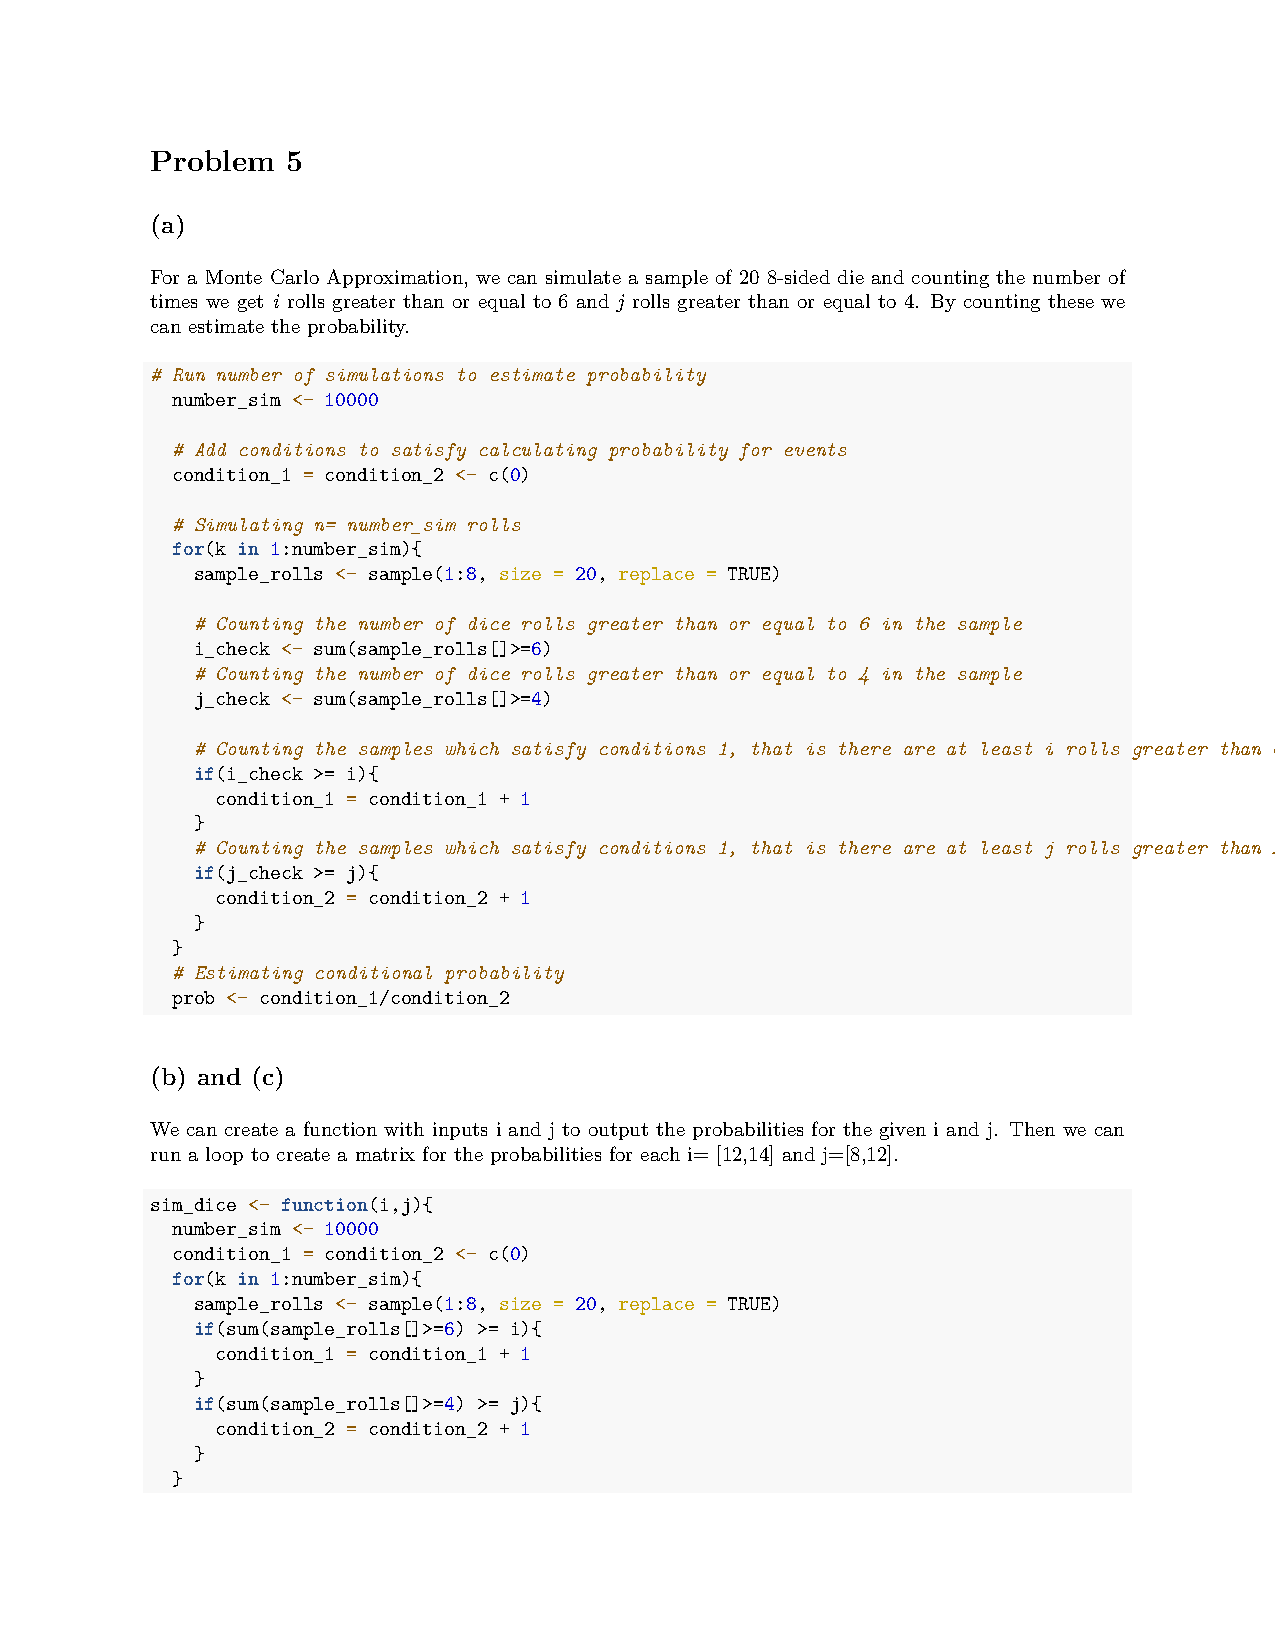
\includepdf[pages=-, pagecommand={}]{Assignment-1-Saksham-Sudershan.pdf}
\end{document}